

\documentclass[5p]{elsarticle}
\usepackage[T1]{fontenc}
\usepackage[utf8]{inputenc}
\usepackage{lmodern}
\usepackage{amsmath}
\usepackage{amsfonts}
\usepackage{amssymb}
\usepackage{graphicx}
\usepackage{float}
\usepackage{placeins}
\usepackage{booktabs}
\usepackage{array}
\usepackage{adjustbox}
\usepackage{url}
\usepackage{xcolor}
\usepackage{tikz}
\usepackage{pdflscape}
\usepackage{microtype}
\usetikzlibrary{positioning,arrows.meta,shapes.geometric,fit,backgrounds,calc}
% --- Workflow-overview figure palette (mirrors the Mermaid version in doc/workflow_overview.md) ---
\definecolor{wfIndigo}{HTML}{312E81}
\definecolor{wfIndigoLight}{HTML}{E0E7FF}
\definecolor{wfIndigoMid}{HTML}{4F46E5}
\definecolor{wfAmberDark}{HTML}{D97706}
\definecolor{wfAmberLight}{HTML}{FEF3C7}
\definecolor{wfAmberText}{HTML}{78350F}
\definecolor{wfEmeraldDark}{HTML}{059669}
\definecolor{wfEmeraldLight}{HTML}{D1FAE5}
\definecolor{wfEmeraldText}{HTML}{064E3B}
\definecolor{wfEmeraldBg}{HTML}{ECFDF5}
\definecolor{wfPinkDark}{HTML}{DB2777}
\definecolor{wfPinkLight}{HTML}{FCE7F3}
\definecolor{wfPinkText}{HTML}{831843}
\definecolor{wfBlueDark}{HTML}{2563EB}
\definecolor{wfBlueLight}{HTML}{DBEAFE}
\definecolor{wfBlueText}{HTML}{1E3A8A}
\definecolor{wfBlueBg}{HTML}{EFF6FF}
\definecolor{wfViolet}{HTML}{7C3AED}
\definecolor{wfVioletDark}{HTML}{5B21B6}
\definecolor{wfRoseDark}{HTML}{E11D48}
\definecolor{wfRoseLight}{HTML}{FFE4E6}
\definecolor{wfRoseText}{HTML}{881337}
\definecolor{wfRoseBg}{HTML}{FFF1F2}
\definecolor{wfSlate}{HTML}{475569}
\newcolumntype{L}[1]{>{\raggedright\arraybackslash}p{#1}}

\newcommand{\widecomparisonplot}[1]{\includegraphics[width=0.76\textwidth]{#1}}

\newcommand{\encodingexampleplot}[1]{\includegraphics[width=0.42\linewidth]{#1}}
\newcommand{\subfigtext}[1]{\par\smallskip{\footnotesize #1\par}}
\setlength{\textfloatsep}{8pt plus 2pt minus 2pt}
\setlength{\floatsep}{8pt plus 2pt minus 2pt}
\setlength{\intextsep}{8pt plus 2pt minus 2pt}
\raggedbottom
\hyphenation{op-tical net-works semi-conduc-tor}


\begin{document}

\begin{frontmatter}

\title{Controlled Reconstruction of Image-Based Time-Series Encodings: Operational Decoders for GAF, RP, and MTF Representations}

\author[mydass]{Adriano García-Giralda Milena}
\author[cls]{Francisco García Moreno}
\author[alg]{José Antonio Jiménez Madrid}
\author[cls]{María Bermúdez Edo}

\affiliation[mydass]{organization={MYDASS Research Group, University of Granada}, country={Spain}}
\affiliation[cls]{organization={Department of Computer Languages and Systems, University of Granada}, country={Spain}}
\affiliation[alg]{organization={Department of Algebra, University of Granada}, country={Spain}}







\begin{abstract}
Image-based time-series encodings expose temporal structure to image-domain models, but their usefulness for signal generation depends on whether the encoded image can be mapped back to the time domain. We study this controlled reconstruction problem for Recurrence Plots (RP), Gramian Angular Summation and Difference Fields (GASF/GADF), and Markov Transition Fields (MTF). We propose two faithful decoders: a signed-RP decoder based on two-dimensional classical multidimensional scaling, adjacent-state overlap, and signed orientation selection; and a closed-form, restricted-branch GADF decoder with image-derived boundary anchoring and multi-pivot averaging. The established GASF diagonal inverse is the invertible baseline. Because MTF is many-to-one, its Fiedler-ordered output is evaluated only as a best-effort representative decoder and lossy control.

On 8,172 triaxial WISDM windows we organise the evaluation as a hierarchy of \emph{fidelity}, \emph{robustness}, and \emph{utility}. Fidelity separates spectral shape from total energy; utility asks whether subject-level accuracy is equivalent within a one-percentage-point margin. Under their explicitly stated decoder contracts (RP additionally consuming its per-window operator range), RP, GASF, and GADF form a near-original fidelity tier over all 8,172 windows, with global mean MAEs of 0.0148, 0.0205, and 0.0157\,m/s$^2$; their mean Pearson correlations are approximately one, mean PSD-shape distances below 0.01, and mean dominant-frequency errors below 0.01\,Hz. Under the primary grouped subject-out three-fold classification protocol, simultaneous subject-cluster bootstrap intervals then place all six classifier-specific accuracy differences within the equivalence region. These are mean results with the reported between-window dispersion, not per-window bounds. MTF is consistently lossy. A repeated Gaussian-noise experiment is interpreted only as a controlled local-stability stress test; genuinely generated images remain unevaluated.
\end{abstract}

\begin{keyword}
Markov Transition Fields \sep Recurrence Plots \sep Gramian Angular Fields \sep Gramian Angular Difference Field \sep Time Series Reconstruction \sep Image Encoding \sep Accelerometer Data \sep Machine Learning
\end{keyword}

\end{frontmatter}




\section{Introduction}
\label{sec:introduction}
Time-series images such as Recurrence Plots (RP), Markov Transition Fields (MTF), and Gramian Angular Fields (GAF) allow image-domain models to operate on temporal relations rather than directly on raw samples \cite{wang2015encoding,wang2015encoding2}. For triaxial accelerometer windows, each axis is encoded separately and stored as one image channel. This representation is attractive for image generation, but it raises a prerequisite question: does an encoded image retain enough information to recover the underlying signal?

We address that reconstruction problem under controlled conditions. Every evaluated image is the deterministic output of a known encoder; encoder settings are known, RP additionally receives the stored operator range required by the current PNG mapping, and per-window amplitude calibration is used only when reconstruction in physical units is requested. We do not train a diffusion model or a GAN, and we make no claim that an arbitrary generated image is automatically physically valid. Instead, we establish which representations can return faithfully to the time domain before generative augmentation is attempted.

The study compares four encodings under one protocol, organised into three blocks --- fidelity (range-normalised pointwise error and a spectral lens), robustness (decoding perturbed and re-encoded images), and utility (subject-level equivalence of six original-trained classifiers). Both stratified window-level and grouped subject-out three-fold splits are reported on the WISDM smartwatch accelerometer data. Figure~\ref{fig:workflow_overview} summarises the workflow, and Table~\ref{tab:decoder_contract} declares each decoder's input/output contract.

The main contributions are:

\begin{itemize}
    \item a signed-RP decoder for continuous Lu--Tong recurrence plots of overlapping states, combining two-dimensional classical multidimensional scaling, consecutive-state overlap alignment, and signed orientation selection;

    \item a closed-form GADF decoder whose restricted angular branch, image-derived boundary anchor, and multi-pivot reconstruction make the normalised inverse operational without method-specific per-window metadata;
    \item a controlled comparison against the prior-art GASF diagonal inverse and a Fiedler-vector MTF representative decoder, explicitly treated as a lossy control rather than a true inverse; and
    \item a validation framework organised as fidelity, robustness, and utility --- including range-normalised local-change error, separate spectral-shape and energy errors, a repeated local perturbation test, and simultaneous subject-cluster equivalence intervals --- under which RP, GASF, and GADF reconstruct near the 8-bit quantisation floor, whereas MTF remains lossy.
\end{itemize}

\begin{figure*}[!htbp]
\centering
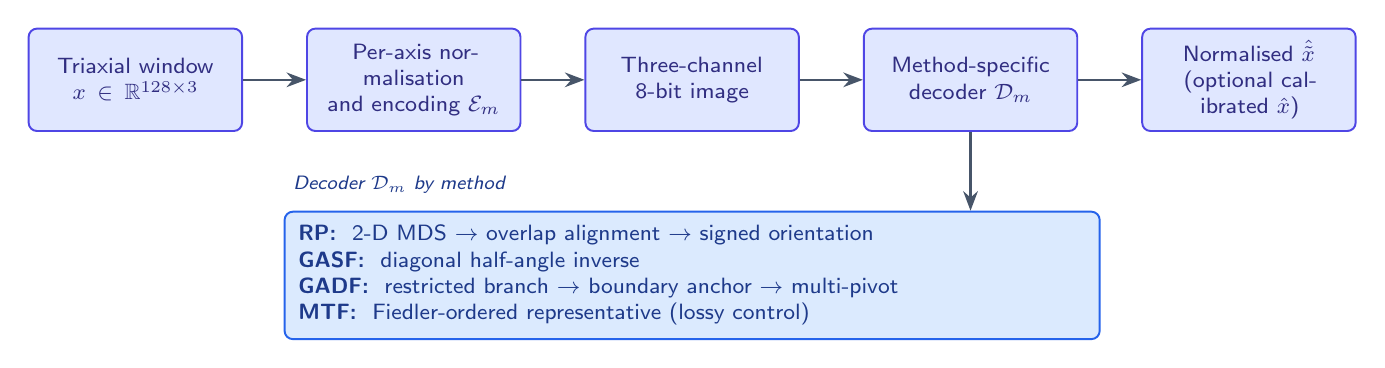
\begin{tikzpicture}[
  font=\sffamily\footnotesize,
  node distance=8mm,
  box/.style={rectangle, rounded corners=3pt, draw=wfIndigoMid, line width=0.7pt,
              fill=wfIndigoLight, text=wfIndigo, align=center,
              minimum height=13mm, text width=2.5cm, inner sep=3pt},
  detail/.style={rectangle, rounded corners=3pt, draw=wfBlueDark, line width=0.7pt,
                 fill=wfBlueLight, text=wfBlueText, align=left,
                 minimum height=9mm, text width=10cm, inner sep=5pt},
  dlabel/.style={text=wfBlueText, font=\sffamily\scriptsize\itshape},
  arrow/.style={->, draw=wfSlate, line width=0.9pt, >=Stealth}
]
  \node[box] (input) {Triaxial window\\$x\in\mathbb{R}^{128\times3}$};
  \node[box, right=of input] (encode) {Per-axis normalisation\\and encoding $\mathcal E_m$};
  \node[box, right=of encode] (image) {Three-channel\\8-bit image};
  \node[box, right=of image] (decode) {Method-specific\\decoder $\mathcal D_m$};
  \node[box, right=of decode] (output) {Normalised $\hat{\tilde x}$\\(optional calibrated $\hat x$)};
  \draw[arrow] (input) -- (encode);
  \draw[arrow] (encode) -- (image);
  \draw[arrow] (image) -- (decode);
  \draw[arrow] (decode) -- (output);

  \node[detail, below=10mm of image] (methods) {%
    \textbf{RP:}~~2-D MDS $\to$ overlap alignment $\to$ signed orientation\\
    \textbf{GASF:}~~diagonal half-angle inverse\\
    \textbf{GADF:}~~restricted branch $\to$ boundary anchor $\to$ multi-pivot\\
    \textbf{MTF:}~~Fiedler-ordered representative (lossy control)};
  \node[dlabel, above=1mm of methods.north west, anchor=south west] {Decoder $\mathcal D_m$ by method};
  \draw[arrow] (decode.south) -- (decode.south |- methods.north);
\end{tikzpicture}
\caption{Controlled reconstruction workflow. Each axis is normalised, encoded, and stored as an 8-bit image channel, then decoded in its method-specific normalised domain and optionally returned to physical units with per-axis calibration. The lower box expands the method-specific decoder $\mathcal D_m$.}
\label{fig:workflow_overview}
\end{figure*}

\section{Related Work and Encodings}
\label{sec:related_encodings}

\subsection{Time-series imaging}
Encoding a one-dimensional signal as a two-dimensional image lets vision architectures operate explicitly on pairwise temporal relations that sequence models must otherwise learn from the raw temporal representation. Wang and Oates introduced this idea for time-series classification and imputation, mapping each window to Gramian angular fields and Markov transition fields before applying convolutional networks \cite{wang2015encoding,wang2015encoding2}. Recurrence plots predate that line as a tool for visualising the recurrences of a dynamical system \cite{eckmann1995recurrence,marwan2007recurrence} and were later adopted as image inputs for the same reason: a single frame exposes global pairwise structure --- distances, periodicities, and symmetries --- that is only implicit in the raw samples.

Since then, image encodings have been applied across several time-series tasks. In human activity recognition, inertial signals have been transformed into GAF, MTF, RP, and related image representations so that convolutional vision architectures can be used for feature extraction \cite{ahmad2021inertial}. GAF-based representations have also been employed for multivariate anomaly detection by expressing temporal and inter-sensor relationships as spatial image patterns \cite{ma2024anomaly}, as well as for missing-value imputation \cite{huamin2020reconstruction}. More recently, image-domain generative models have been used to generate or complete time series through invertible two-dimensional representations, including GASF-based traffic imputation \cite{huang2023tsdigan} and image-based GAN generation followed by explicit inversion to the temporal domain \cite{hellermann2026imagegan}.

These applications exploit the ability of two-dimensional encodings to expose pairwise temporal relations as spatial patterns that convolutional and image-based generative models can process. Their success in a discriminative or generative task, however, does not by itself establish that the original waveform is preserved: a representation can be excellent at predicting an activity label while discarding the amplitude, phase, or ordering information needed to recover it. Whether the map from signal to image can be run backwards is a property distinct from whether the image is useful for classification --- and it is the property on which any image-domain generator ultimately depends.

\subsection{Prior reconstruction methods}
\label{sec:prior_reconstruction}
Three tasks are easily conflated: classification maps an image to a label, reconstruction recovers the signal that produced the image, and image-domain generation synthesises new images that must still map back to valid signals. The latter two require a sufficiently well-defined image-to-signal mapping, with exact invertibility providing the strongest controlled case. Reconstruction is therefore a prerequisite for the image-domain generation workflow considered here. We study the controlled case first and review here what is known about inverting each encoding.

Reconstruction from a time-series image depends on the information retained by the particular encoding. For GASF, Wang and Oates showed that a signal scaled to $[0,1]$ can be recovered directly from the main diagonal,
\[
\tilde x_i=\sqrt{\tfrac{G^{\mathrm S}_{ii}+1}{2}},
\]
because the angular branch is restricted to $\phi_i\in[0,\pi/2]$ \cite{wang2015encoding}. Wang and Oates also demonstrated GASF image recovery for time-series imputation using a denoising autoencoder before applying the diagonal inverse \cite{wang2015encoding}. Later work extended two-dimensional denoising-based reconstruction strategies \cite{huamin2020reconstruction}. This establishes GASF as an operational invertible baseline under a fixed branch. Wang and Oates also stated that GADF on restricted data admits an accurate inverse map, but did not provide an explicit decoder resolving the sine branch, the global angular offset, and image quantisation; their implemented recovery pipeline instead relies on the GASF diagonal.

Reconstruction from recurrence information has followed two main routes. Hirata et al.\ convert a thresholded recurrence plot into a weighted recurrence graph, estimate pairwise distances through graph paths, and apply multidimensional scaling to reproduce the topological shape of the underlying trajectory \cite{hirata2008reproduction}. Sipers et al.\ study the information content and uniqueness conditions of unthresholded recurrence plots generated by time-delay embeddings, and formulate signal reconstruction as a minimisation problem \cite{sipers2011unique}; a later extension considers disturbances and multi-level recurrence information \cite{sipers2017robust}. These methods establish that recurrence information can support geometric or signal reconstruction, but they address unsigned recurrence representations.

The present RP differs in three consequential respects. First, its magnitude already provides the dense Euclidean distance matrix between adjacent states $s_i=(x_i,x_{i+1})$; applying a graph-geodesic reconstruction pipeline would therefore require first reducing this continuous metric information to a recurrence graph, an unnecessary step for the operator considered here. Second, an MDS embedding remains undetermined up to an orthogonal transformation; recovering a scalar sequence therefore requires explicitly enforcing the consecutive-state overlap $s_{i,2}=s_{i+1,1}$. Third, the Lu--Tong sign convention carries directional information that is absent from unsigned RP and URP reconstruction methods, and is used here to select the remaining reflected orientation. Consequently, earlier RP reconstruction methods provide geometric precedents, but cannot be applied unchanged as a decoder for the continuous signed adjacent-state operator used in this work.

MTF presents a different limitation. Quantile assignment removes within-bin amplitudes, and samples belonging to the same state share a transition profile. Wang and Oates consequently observed that recovering a signal from MTF is highly uncertain compared with GAF \cite{wang2015encoding}. To the best of our knowledge, no exact MTF-to-series inverse has been reported; image-restoration work on Markov random fields addresses a different problem \cite{kopec1994document,kliewer2006iterative}. The spectral-seriation procedure considered here therefore returns only a representative quantile trajectory and is evaluated as a lossy control.

\subsection{Encodings and operators}
RP, GAF, and MTF all map a one-dimensional sequence to a matrix of pairwise temporal relations, but they preserve different information. RP represents phase-space distances or recurrences \cite{eckmann1995recurrence,marwan2007recurrence}; GASF and GADF represent angular sums and differences \cite{wang2015encoding}; and MTF represents transition probabilities between quantised amplitude states \cite{wang2015encoding2}. Table~\ref{tab:operator_summary} summarises the operators and their reconstruction character; prior reconstruction work is discussed in Section~\ref{sec:prior_reconstruction}.

\begin{table}[!htbp]
\centering
\caption{Encodings and their reconstruction character.}
\label{tab:operator_summary}
\small
\setlength{\tabcolsep}{4pt}
\begin{tabular}{@{}L{0.17\columnwidth}L{0.30\columnwidth}L{0.45\columnwidth}@{}}
\toprule
Method & Operator & Reconstruction character \\
\midrule
RP & signed \(\lVert s_i-s_j\rVert_2\) & Recoverable under distance-scale, overlap, and signed-orientation assumptions \\
GASF & \(\cos(\phi_i+\phi_j)\) & Closed-form recovery on a fixed branch \\
GADF & \(\sin(\phi_i-\phi_j)\) & Closed-form recovery under branch and anchor assumptions \\
MTF & \(W_{q_i,q_j}\) & Non-invertible; representative trajectory only \\
\bottomrule
\end{tabular}
\end{table}

\begin{figure*}[!htbp]
\centering
\begin{minipage}[t]{0.24\linewidth}
\centering
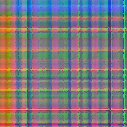
\includegraphics[width=\linewidth]{images/1600xtrp0.png}
\subfigtext{(a) RP}
\end{minipage}\hfill
\begin{minipage}[t]{0.24\linewidth}
\centering
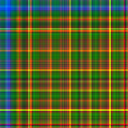
\includegraphics[width=\linewidth]{images/1600x0tgasf.png}
\subfigtext{(b) GASF}
\end{minipage}\hfill
\begin{minipage}[t]{0.24\linewidth}
\centering
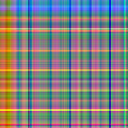
\includegraphics[width=\linewidth]{images/1600x0tgadf.png}
\subfigtext{(c) GADF}
\end{minipage}\hfill
\begin{minipage}[t]{0.24\linewidth}
\centering
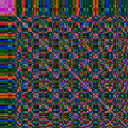
\includegraphics[width=\linewidth]{images/1600x0tmtf.png}
\subfigtext{(d) MTF}
\end{minipage}
\caption{The four image encodings of one triaxial WISDM walking window, with the per-axis $(x,y,z)$ intensities stacked as the RGB channels. RP encodes signed recurrence distances between adjacent states; GASF is symmetric; GADF is antisymmetric and therefore directional; and MTF shows the discrete transition-level regions of its quantised states. RP is $127\times127$ (adjacent-state embedding) and the others $128\times128$. The reconstructions of this same window are shown in Figure~\ref{fig:qualitative_main}.}
\label{fig:encodings_main}
\end{figure*}

\subsection{Recurrence plots}
Following delay-coordinate embedding \cite{takens1981detecting}, a scalar series is represented by states \(s_i=(x_i,x_{i+1})\in\mathbb{R}^2\), giving \(N-1\) overlapping states for a window of length \(N\). Classical recurrence plots then threshold pairwise state distances \cite{eckmann1995recurrence,marwan2007recurrence} and are therefore invariant to orientation. We instead use the continuous Lu--Tong construction \cite{lu2019robust}, with reference direction \(v=(1,1)^\top/\sqrt{2}\):
\begin{equation}
R_{ij}=\sigma(i,j)\lVert s_i-s_j\rVert_2,
\label{eq:FormulaRP}
\end{equation}
where, writing $\hat u_{ij}=(s_i-s_j)/\lVert s_i-s_j\rVert_2$ for the unit displacement when $\lVert s_i-s_j\rVert_2>0$,
\begin{equation}
\sigma(i,j)=
\begin{cases}
-1,& \lVert s_i-s_j\rVert_2>0\ \text{and}\ \hat u_{ij}\cdot v<\cos(3\pi/4),\\
1,&\text{otherwise}.
\end{cases}
\end{equation}
The magnitude contains the two-dimensional Euclidean geometry of the adjacent states; the sign supplies an orientation cue. Prior recurrence-reconstruction methods, and how our decoder departs from them, are discussed in Section~\ref{sec:prior_reconstruction}.

\subsection{Gramian angular fields}
After normalisation, samples are mapped to angles \(\phi_i=\arccos(\tilde{x}_i)\). The two GAF variants are
\begin{align}
G^{\mathrm{S}}_{ij}
 &=\cos(\phi_i+\phi_j)
 =\tilde{x}_i\tilde{x}_j-\sqrt{1-\tilde{x}_i^2}\sqrt{1-\tilde{x}_j^2},
 \label{eq:gasf_indexed}\\
G^{\mathrm{D}}_{ij}
 &=\sin(\phi_i-\phi_j)
 =\sqrt{1-\tilde{x}_i^2}\tilde{x}_j-\tilde{x}_i\sqrt{1-\tilde{x}_j^2}.
 \label{eq:gadf_indexed}
\end{align}
GASF exposes sample magnitude through \(G^{\mathrm{S}}_{ii}=\cos(2\phi_i)\), which supports the known diagonal inverse on \(\phi_i\in[0,\pi/2]\). GADF has an identically zero diagonal and retains only relative angular differences. Its inverse must therefore choose an \(\arcsin\) branch and fix a global angular offset; Section~\ref{sec:gadf_reconstruction_proposal} supplies both.

\subsection{Markov transition fields}
\label{sec:mtf_definition}
MTF assigns each sample to one of \(Q\) quantile states \(q_t\) and estimates
\[
W_{p,q}=P(q_{t+1}=q\mid q_t=p).
\]
The image expands this \(Q\times Q\) matrix to the time grid,
\[
M_{a,b}=W_{q_a,q_b},\qquad a,b=1,\ldots,N.
\]
All samples in the same bin share a transition profile, so MTF can preserve coarse dynamics while discarding within-bin amplitude and the global orientation of the amplitude order. Its decoded trajectory is consequently a representative, not an inverse.

\subsection{Research gap}
\label{sec:research_gap}
Two gaps follow. To the best of our knowledge, no operational decoder has been reported for restricted-branch GADF or for the continuous signed adjacent-state RP considered here, particularly after finite-precision image storage. Likewise, we are not aware of a controlled comparison of these four encodings spanning reconstruction fidelity, perturbation stability, and downstream utility. This work proposes operational GADF and signed-RP decoders and evaluates them within such a common protocol, using GASF as the prior-art invertible baseline and MTF as a lossy control.

\section{Problem Formulation}
\label{sec:problem_formulation}


Let \(x=(x_1,\ldots,x_N)\) denote one axis of an accelerometer window. Method \(m\) applies a normaliser \(\mathcal N_m\), an encoder \(\mathcal E_m\), and a decoder \(\mathcal D_m\):
\[
\tilde x^{(m)}=\mathcal N_m(x),\qquad
M^{(m)}=\mathcal E_m(\tilde x^{(m)}),
\]
\[
\hat{\tilde x}^{(m)}=\mathcal D_m(M^{(m)}).
\]
Here \(M^{(m)}\in\mathbb R^{N_m\times N_m}\), with \(N_m=N\) for GASF, GADF, and MTF and \(N_m=N-1\) for the adjacent-state RP. The primary reconstruction problem is to recover the normalised signal \(\hat{\tilde x}^{(m)}\); returning to physical units,
\[
\hat x=\mathcal N_m^{-1}(\hat{\tilde x}^{(m)};x_{\min},x_{\max}),
\]
is a common optional calibration step. Each accelerometer axis is encoded independently, stored as one RGB channel, decoded, and regrouped into a triaxial window.

\section{Proposed Reconstruction Methods}
\label{sec:proposed_methods}

\subsection{Shared normalisation and storage protocol}
\label{sec:shared_protocol}

Encoded matrices are stored and reread as 8-bit PNG images. RP and both Gramian fields are min--max mapped to \([0,255]\); MTF already occupies \([0,1]\). Table~\ref{tab:decoder_contract} separates information required for normalised reconstruction from the optional amplitude calibration used for physical units.

\begin{table*}[!htbp]
\centering
\caption{Decoder outputs and the method-specific per-window information required under the current storage protocol. Fixed encoder conventions are assumed known.}
\label{tab:decoder_contract}
\small
\setlength{\tabcolsep}{6pt}
\begin{tabular}{@{}L{0.12\textwidth}L{0.38\textwidth}L{0.40\textwidth}@{}}
\toprule
Method & Decoder output & Required per-window information \\
\midrule
RP   & Normalised waveform & $(R_{\min},R_{\max})$ under the current PNG mapping \\
GASF & Normalised waveform in $[0,1]$ & None \\
GADF & Normalised waveform in $[-\alpha,\alpha]$ & None \\
MTF  & Quantile-level representative trajectory & None \\
\bottomrule
\end{tabular}

\smallskip
\footnotesize
MTF does not provide a true inverse. Returning any decoded output to the observed signal scale additionally requires the common per-axis calibration $(x_{\min},x_{\max})$.
\end{table*}

Under the current storage protocol, RP is the only decoder requiring method-specific per-window information: the min--max PNG mapping removes the scale of its signed distance matrix, which must be restored through \((R_{\min},R_{\max})\) before MDS. This operator range is distinct from the common amplitude calibration \((x_{\min},x_{\max})\), which is used only to return a decoded normalised trajectory to the observed physical scale. Consequently, the headline results compare the methods under their declared decoder contracts rather than under identical side information. This RP dependence arises largely from the current per-window storage convention and could be removed through a fixed dataset-wide RP range, at the cost of lower 8-bit resolution for low-amplitude windows (Section~\ref{sec:disc_scope}). For GADF, the small difference between its theoretical range and the fixed \([-1,1]\) PNG mapping is analysed separately in the Supplementary Material.

\subsection{Signed recurrence-plot decoder}
\label{sec:rp_reconstruction_method}

For the continuous signed RP in Equation~\ref{eq:FormulaRP}, the magnitude matrix contains Euclidean distances between adjacent states \(s_i=(x_i,x_{i+1})\). The proposed decoder recovers their full two-dimensional geometry and fixes the orthogonal ambiguity using overlap and sign:


\begin{enumerate}
\item Invert PNG storage with the RP matrix range \([R_{\min},R_{\max}]\). Form the symmetric distance matrix
\[
D_{ij}=\tfrac12\bigl(|R^{\mathrm{obs}}_{ij}|+|R^{\mathrm{obs}}_{ji}|\bigr),\qquad D_{ii}=0.
\]
\item Apply classical MDS to \(D\). If \(J=I-\mathbf1\mathbf1^\top/(N-1)\), eigendecomposition of \(-\tfrac12JD^2J\) yields the two leading coordinates \(Y=V_2\Lambda_2^{1/2}\).

\item Search the two-dimensional orthogonal transformations of \(Y\) for the one that minimises the adjacent-state overlap error \(s_{i,2}-s_{i+1,1}\). Among near-minimisers, select the orientation whose regenerated signed RP is closest to \(R^{\mathrm{obs}}\) in Frobenius norm.
\item For aligned states \(\hat s_i=(a_i,b_i)\), recover all \(N\) samples:
\[
\hat x_1=a_1,\qquad
\hat x_i=\tfrac12(b_{i-1}+a_i)\ (2\le i\le N-1),\qquad
\hat x_N=b_{N-1}.
\]
\item Pairwise distances are translation invariant, so map the recovered sequence's minimum and maximum to the known normalised range. Physical-unit recovery, if required, then uses the shared calibration.
\end{enumerate}

Retaining both MDS dimensions is essential because the embedded states are genuinely two-dimensional. The signed comparison resolves the reflection that remains after overlap alignment; Section~\ref{sec:decoder_ablation} summarises both choices.

\subsection{GASF diagonal inverse}
\label{sec:gasf_reconstruction_method}

GASF is the controlled prior-art baseline \cite{wang2015encoding}. On the branch \(\phi_i\in[0,\pi/2]\),
\[
G^{\mathrm S}_{ii}=\cos(2\phi_i),\qquad
\hat\phi_i=\tfrac12\arccos(G^{\mathrm S}_{ii}),\qquad
\hat{\tilde x}_i=\cos(\hat\phi_i).
\]
The branch condition matters: under \([-1,1]\) scaling the diagonal determines only \(|\tilde x_i|\). With the \([0,1]\) protocol used here, the normalised shape follows from the diagonal and the amplitude range is needed only for optional physical-unit recovery.

\subsection{Restricted-branch GADF decoder}
\label{sec:gadf_reconstruction_proposal}

GADF contains relative angles \(G^{\mathrm D}_{ij}=\sin(\phi_i-\phi_j)\) but no diagonal amplitude information. We scale each non-constant window to
\[
\bar x_t=2\alpha\frac{x_t-x_{\min}}{x_{\max}-x_{\min}}-\alpha,
\qquad \alpha=0.7,
\]
so \(\phi_t=\arccos(\bar x_t)\). A unique principal-branch inverse requires
\[
\max_{i,j}|\phi_i-\phi_j|
=\pi-2\arccos(\alpha)<\frac{\pi}{2},
\]
which is equivalent to \(\alpha<1/\sqrt2\). The choice \(\alpha=0.7\) is therefore close to the largest admissible symmetric range while retaining a numerical margin. Under this restriction,
\[
\arcsin(G^{\mathrm D}_{ij})=\phi_i-\phi_j.
\]

A pivot row \(p\) determines all angles relative to \(\phi_p\):

\[
\phi_j=\phi_p-\arcsin(G^{\mathrm D}_{pj}).
\]
The remaining global offset is fixed from the image. Per-window normalisation guarantees samples at both boundaries \(\pm\alpha\). The row mean
\[
\mu_i=\frac1N\sum_jG^{\mathrm D}_{ij}
=\bar C\sin\phi_i-\bar S\cos\phi_i
\]

is strictly increasing over the restricted angular interval. Hence
\[
e=\arg\max_i|\mu_i|
\]
identifies a boundary row, and the sign of \(\mu_e\) selects \(\phi_e=\arccos(-\alpha)\) or \(\arccos(\alpha)\). For each of the \(n_p=5\) rows with the smallest \(|\mu_p|\),
\[
\hat\phi^{(p)}_j
=\phi_e-\arcsin(G^{\mathrm D}_{ep})-\arcsin(G^{\mathrm D}_{pj}),
\qquad
\hat{\bar x}_j=
\cos\left(\frac1{n_p}\sum_{p}\hat\phi^{(p)}_j\right).
\]
Averaging angles over central pivots reduces PNG quantisation noise without changing the \(O(N^2)\) cost of reading the matrix and computing its row means. The inverse is exact in real arithmetic under the branch, boundary, and sign assumptions; it is not a generic inverse for unconstrained GADF images.

\subsection{Best-effort Fiedler-vector MTF representative}
\label{sec:mtf_reconstruction_method}

MTF is many-to-one, so the decoder returns a representative trajectory compatible with its transition structure:

\begin{enumerate}
\item Cluster the \(N\) image rows into \(Q\) groups using farthest-point-initialised \(k\)-means. Equal rows correspond to the same quantile state in a clean MTF.
\item Average image blocks to estimate \(W\), symmetrise it as \(S=(W+W^\top)/2\), and form the graph Laplacian \(L=D-S\).
\item Sort the recovered groups by the Fiedler vector of \(L\), following spectral seriation \cite{Atkins1998}. This recovers the amplitude order for an ideal birth--death chain and is a heuristic for general transition graphs.
\item Assign the midpoint \((k-\tfrac12)/Q\) to samples in ordered group \(k\).
\end{enumerate}

The image does not determine the global reversal of the amplitude order, and all values within a bin share one representative. We use \(Q=4\); the full bin-count and metadata sweeps are reported in the Supplementary Material.
\section{Experimental Protocol}
\label{sec:experimental_protocol}

\subsection{Dataset and segmentation}

We use the 20\,Hz smartwatch accelerometer stream of the WISDM Smartphone and Smartwatch Activity and Biometrics Dataset \cite{misc_wisdm_smartphone_and_smartwatch_activity_and_biometrics_dataset__507}. Five nearly balanced activities are retained: standing (20.6\%), sitting (20.2\%), walking (20.0\%), stairs (19.7\%), and jogging (19.5\%). Within every contiguous subject--activity recording, we form non-overlapping windows of \(N=128\) samples (6.4\,s) and discard the final incomplete block. No window crosses a subject or activity boundary.

This produces 8,172 labelled triaxial windows from 51 subjects, or 24,516 one-axis reconstructions. GASF, GADF, and MTF images are \(128\times128\); the adjacent-state RP is \(127\times127\), and its overlap reconstruction returns 128 samples.

Two complementary three-fold protocols are evaluated. The \emph{window-level} split is class-stratified and may place windows from the same subject in train and test, so it measures reconstruction-induced distribution shift within the observed population. The \emph{grouped subject-out} split assigns all windows from a subject to one fold, holding out disjoint groups of 16, 18, and 17 subjects. It is our \emph{primary} protocol, since it estimates generalisation to unseen individuals; the window-level split is reported only as an optimistic within-distribution reference, and its full comparison is deferred to the Supplementary Material. Because the decoders are deterministic and untrained, reconstruction errors pooled over the three test folds cover the same 8,172 windows under either split; classifier performance differs because a new model is trained for each fold, and the subject-level equivalence result (Table~\ref{tab:equivalence_ci}) is reported under the subject-out protocol.

\subsection{Evaluation design}

The four reconstruction procedures are compared in a hierarchy of three blocks --- fidelity, robustness, and utility --- so that each answers a distinct question and later blocks are interpreted only once earlier ones hold.

\paragraph{Fidelity: signal and spectrum.}
\label{sec:fidelity_metrics}
Time-domain fidelity uses \emph{range-normalised} metrics, so the four encoders are comparable regardless of each window's amplitude. Writing \(r=\max_i x_i-\min_i x_i\) for one axis,
\[
\mathrm{NMAE}=\frac{1}{r\,n}\sum_i|x_i-\hat x_i|,
\]
\[
\mathrm{NRMSE}=\frac{1}{r}\sqrt{\tfrac1n\sum_i(x_i-\hat x_i)^2},
\]
together with Pearson correlation and the range-normalised first-difference error
\[
\Delta\text{-NMAE}=\frac{1}{r(n-1)}\sum_i\bigl|(x_{i+1}-x_i)-(\hat x_{i+1}-\hat x_i)\bigr|,
\]
which checks whether local changes, not only global amplitude, are preserved. When \(r\le\tau_r=10^{-8}\,\mathrm{m/s^2}\), a relative error is numerically undefined; that axis is omitted from range-normalised summaries rather than divided by an arbitrary epsilon. No evaluated window was excluded under this rule. We drop MRE, whose \(|x_i|+\varepsilon\) denominator lets accelerometer zero-crossings dominate.

The spectral lens uses Welch periodograms at \(f_s=20\,\)Hz \cite{Welch1967}. To separate shape from energy, each spectrum is first normalised to unit mass,
\[
p_x(f)=\frac{P_x(f)}{\sum_f P_x(f)+\varepsilon},\qquad
d_{\mathrm{shape}}=\lVert p_x-p_{\hat x}\rVert_1,
\]
while total-energy error is reported separately as
\[
e_E=\frac{|\sum_fP_x(f)-\sum_fP_{\hat x}(f)|}{\sum_fP_x(f)+\varepsilon}.
\]
The main table reports spectral-shape distance and dominant-frequency error; total-energy and band-mass errors are in the Supplementary Material. This lens replaces the previous global cubic-polynomial fit.

\paragraph{Robustness: controlled local stability.}
We sample 150 fold-0 windows, exactly 30 per activity and spread across the available subjects within each activity, drawn with a fixed seed before inspecting any perturbation result so the sample cannot be chosen to favour a method. For every nonzero \(\sigma\in\{2,4,8,16\}\), two independent arrays of zero-mean Gaussian noise are added independently to every pixel and channel of the stored image; intensities are clipped to \([0,255]\), rounded back to integers, and decoded (seed 0). We average replicates within a window and report between-window dispersion and subject-cluster bootstrap intervals. With only two draws per level, the reported dispersion characterises heterogeneity across windows rather than the full noise distribution at any single window; the inference is therefore about between-window variability. This is a controlled local-stability stress test, not a surrogate for generated-image defects.

For the clean image \(I_{m,w}\), the cycle residual is
\[
c_{m,w}=\frac{\sum_{a=1}^{3}\lVert \mathcal E_m(\hat x^{(0)}_{m,w,a})-M_{m,w,a}\rVert_F}
{\sum_{a=1}^{3}\lVert M_{m,w,a}\rVert_F+\varepsilon},
\]
where \(M_{m,w,a}\) is the native float operator matrix that produced image channel \(a\). The wiring gate compares the newly computed clean reconstruction \(\hat x^{(0)}_{m,w}\) with the corresponding cached pipeline reconstruction \(\hat x^{\mathrm{cache}}_{m,w}\): every sampled window must have mean axis-wise NMAE below 0.05. All four methods passed this gate on every sampled window. Cycle details and the float/PNG error decomposition are reported in the Supplementary Material.

\paragraph{Utility: downstream classification.}
Six classifiers are trained once per fold on original triaxial windows; three representative models spanning the families are reported in the body (CNN, GRU, and Random Forest --- convolutional, recurrent, and classical), and all six appear in the Supplementary Material. The same fitted model is then evaluated on the original and on each reconstruction of the held-out windows, a distribution-shift test. We frame utility as an \emph{equivalence} question --- whether reconstruction accuracy lies within a practically negligible margin of the original --- rather than as a difference test. A transfer matrix that trains and evaluates across original and reconstructed data (and their mixture), which would test augmentation directly, is left to future work.

\subsection{Statistical protocol}
\label{sec:statistical_protocol}

All comparisons are paired. Pointwise MAE uses Wilcoxon signed-rank tests \cite{Wilcoxon1945}; a subject-clustered analysis repeats the comparison after reducing each subject to one mean. Window-wise classifier correctness uses continuity-corrected McNemar tests \cite{McNemar1947} as a secondary diagnostic.

The primary utility inference uses the per-subject accuracy difference (Original minus reconstruction). We jointly resample the 51 subjects \(10^4\) times and construct simultaneous \(95\%\) max-deviation bootstrap intervals over one family of 18 subject-out comparisons (six classifiers by RP/GASF/GADF) \cite{DavisonHinkley1997}. The six MTF negative-control comparisons form a separate family. Equivalence requires the entire classifier-specific simultaneous interval to lie within \(\pm0.01\). One percentage point is the primary practical margin because it is too small to alter the method ranking and is well below the observed subject-out fold variation; margin choice remains a substantive judgement \cite{Lakens2017}. The wider \(\pm0.02\) region is a less stringent sensitivity analysis, not a conservative alternative. Paired two one-sided tests (TOST) provide confirmation \cite{Schuirmann1987}: at \(\alpha=0.05\), TOST corresponds to a bilateral \(90\%\) interval, so the simultaneous \(95\%\) bootstrap criterion is the stricter headline rule.

For the confirmatory TOST and difference tests, Holm--Bonferroni controls family-wise \(\alpha=0.05\) separately over the 24 original-versus-reconstruction comparisons, the 36 between-encoder comparisons, and the six pointwise-error pairs \cite{Holm1979}. The window-level protocol repeats these as separate secondary families in the Supplementary Material; neither tests nor intervals are pooled across protocols.

\paragraph{Configuration and internal validity.}
For the subject-out numbers to estimate generalisation to unseen individuals, settings supporting the primary RP/GASF/GADF claims are fixed across folds: classifier hyperparameters and the 20-epoch training budget are unchanged. The classifier architectures and hyperparameters (listed in the Supplementary Material) are standard library defaults fixed before the grouped subject-out evaluation and were not selected using any outer-fold test prediction; no classifier hyperparameter search was run. In addition, per-window normalisation is deterministic; \(\alpha=0.7\) follows from the analytic bound \(\alpha<1/\sqrt2\); and \(n_p=5\) is held fixed. The exception is MTF's \(Q=4\), selected in an exploratory pooled-test sweep. Consequently, MTF is retained only as a descriptive lossy control: we do not claim an unbiased estimate of an optimally tuned MTF decoder. Confirmatory comparison of MTF configurations would require a subject-grouped inner loop inside every outer fold. This limitation cannot affect the confirmatory conclusions for RP, GASF, or GADF, whose settings were not selected by that sweep.
\section{Results}
\label{sec:results}

\subsection{Qualitative reconstruction}

Figure~\ref{fig:qualitative_main} compares the four reconstructions for the same WISDM walking window. RP, GASF, and GADF almost completely overlap the original on all axes. MTF retains coarse temporal structure but replaces continuous amplitude variation with quantile-level plateaus. Synthetic controls, additional encoded-image examples, inversion-sensitivity panels, and per-axis MTF plots are provided in the Supplementary Material.

\begin{figure*}[!t]
\centering
\begin{minipage}[t]{0.48\linewidth}
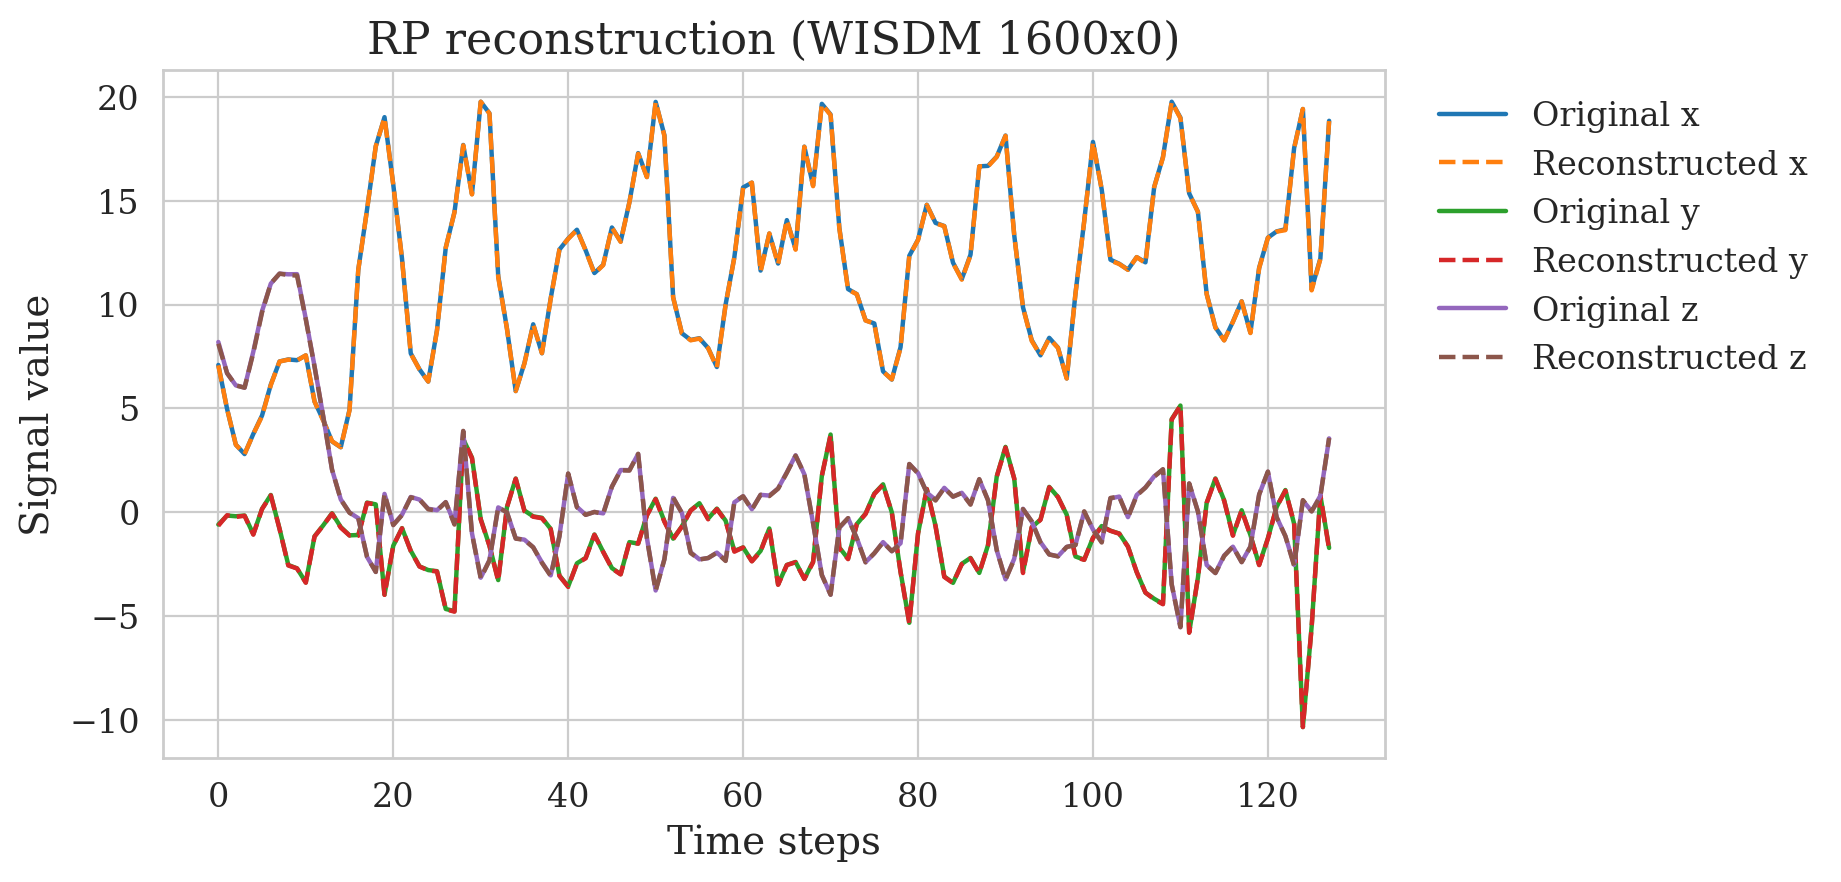
\includegraphics[width=\linewidth]{images/rp_sample_0_global.png}
\subfigtext{(a) RP}
\end{minipage}\hfill
\begin{minipage}[t]{0.48\linewidth}
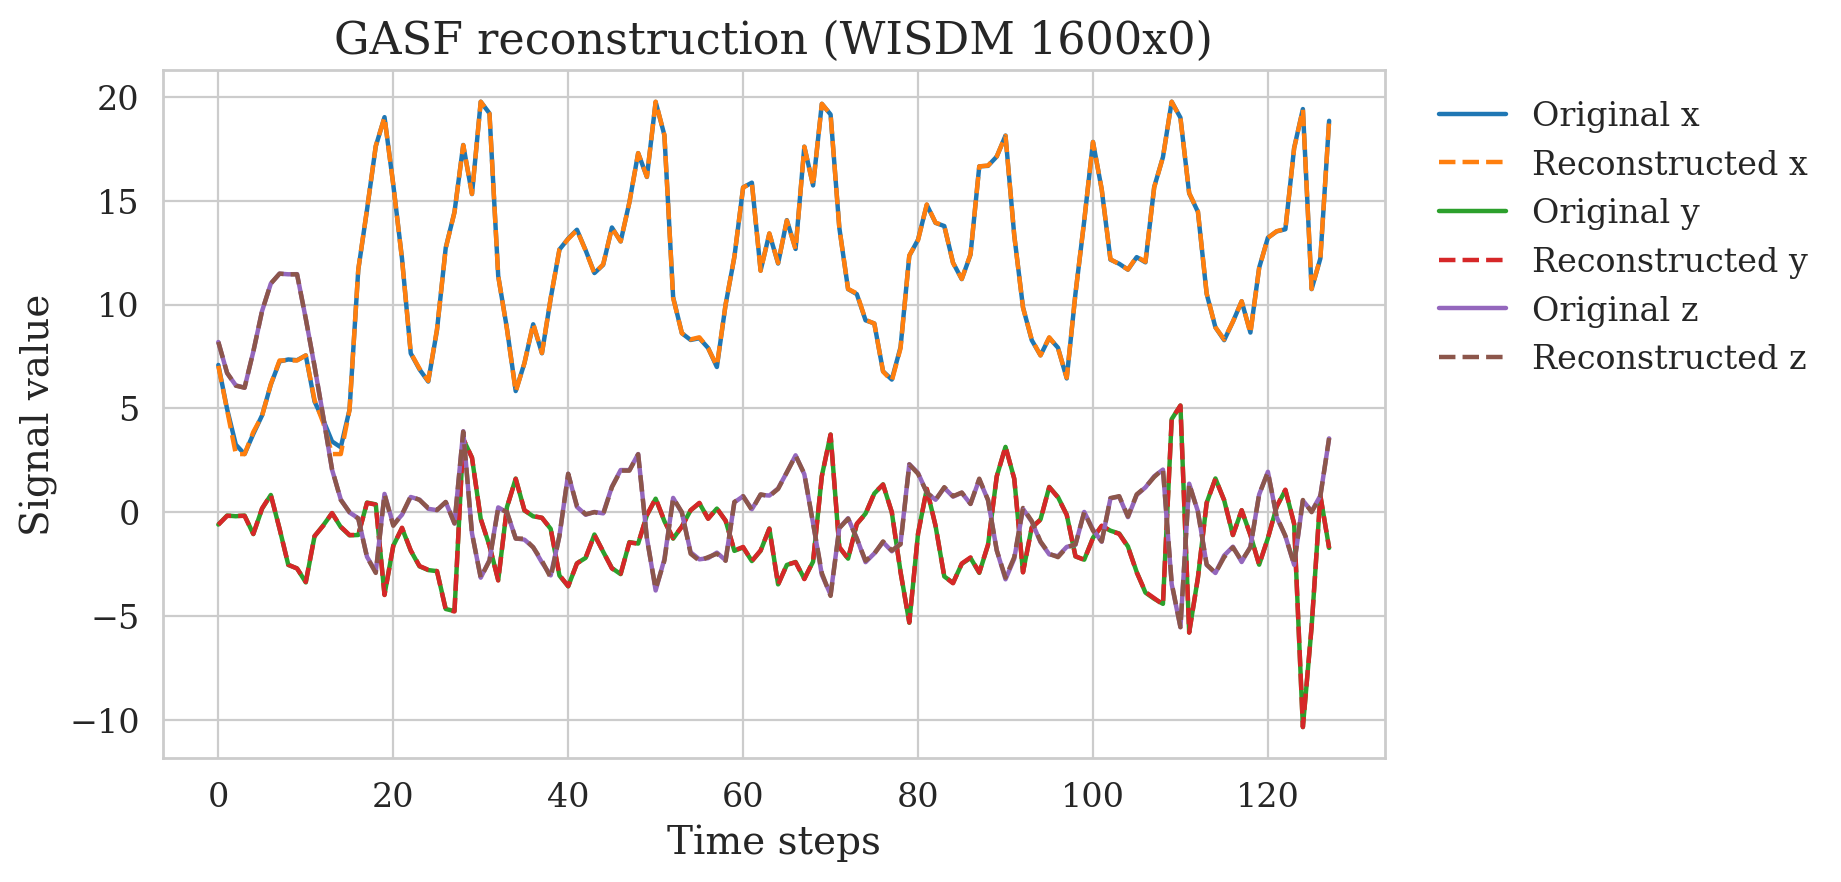
\includegraphics[width=\linewidth]{images/gaf_sample_0_global.png}
\subfigtext{(b) GASF}
\end{minipage}

\begin{minipage}[t]{0.48\linewidth}
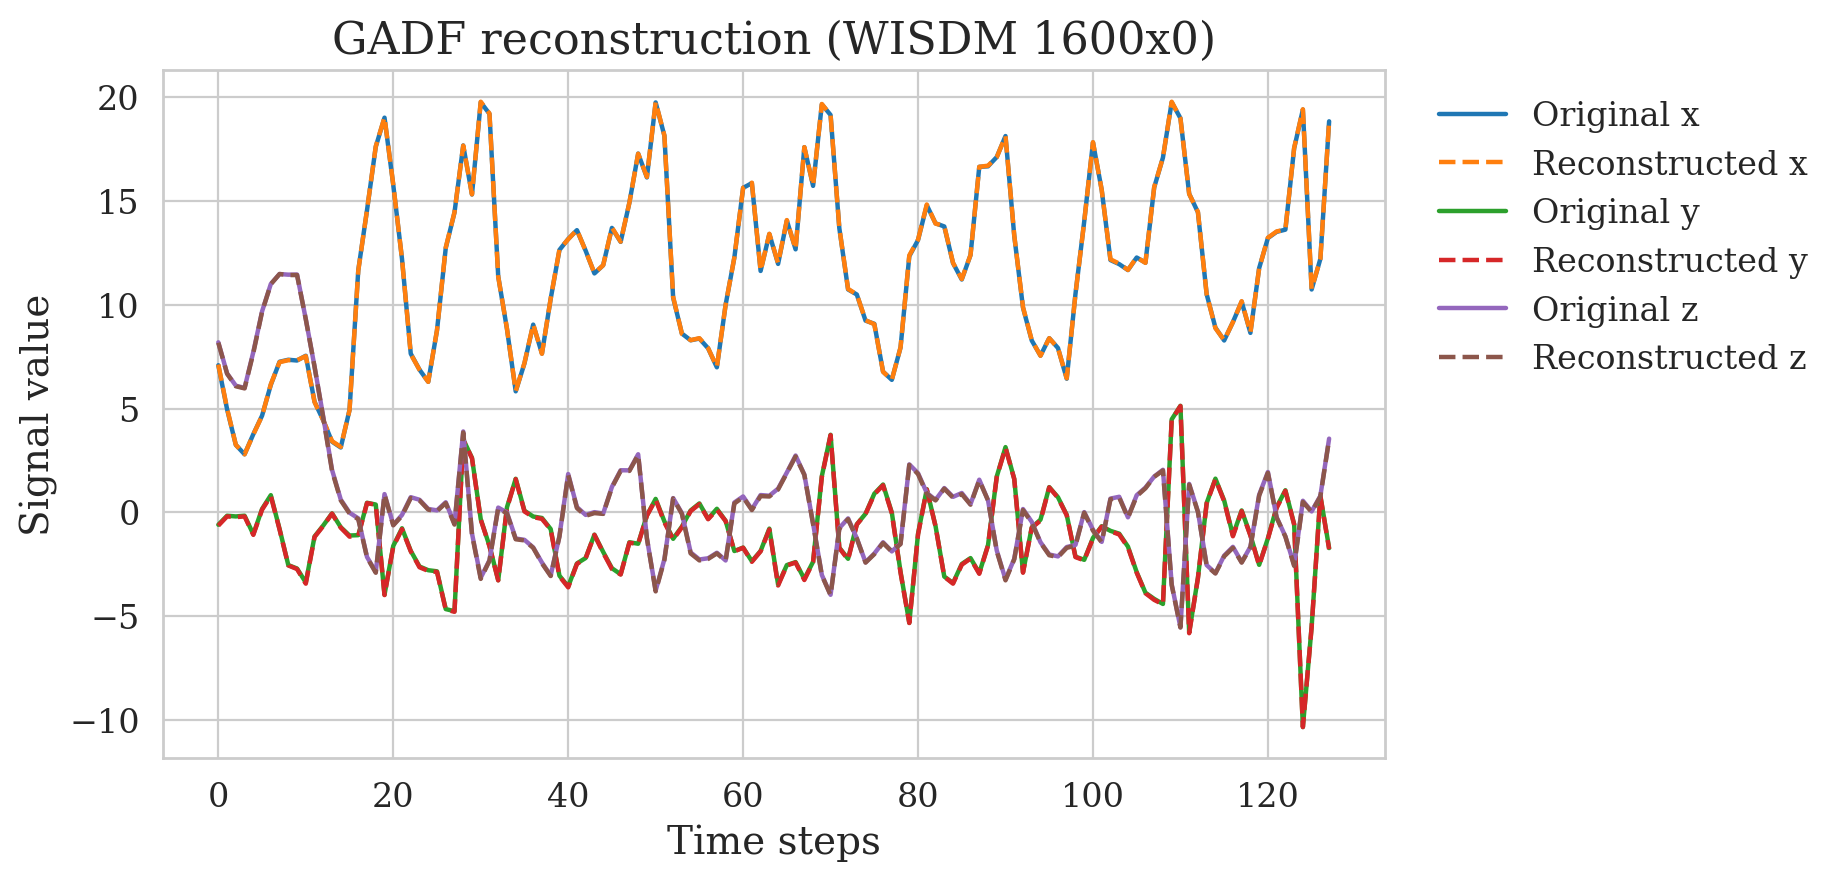
\includegraphics[width=\linewidth]{images/gadf_sample_0_global.png}
\subfigtext{(c) GADF}
\end{minipage}\hfill
\begin{minipage}[t]{0.48\linewidth}
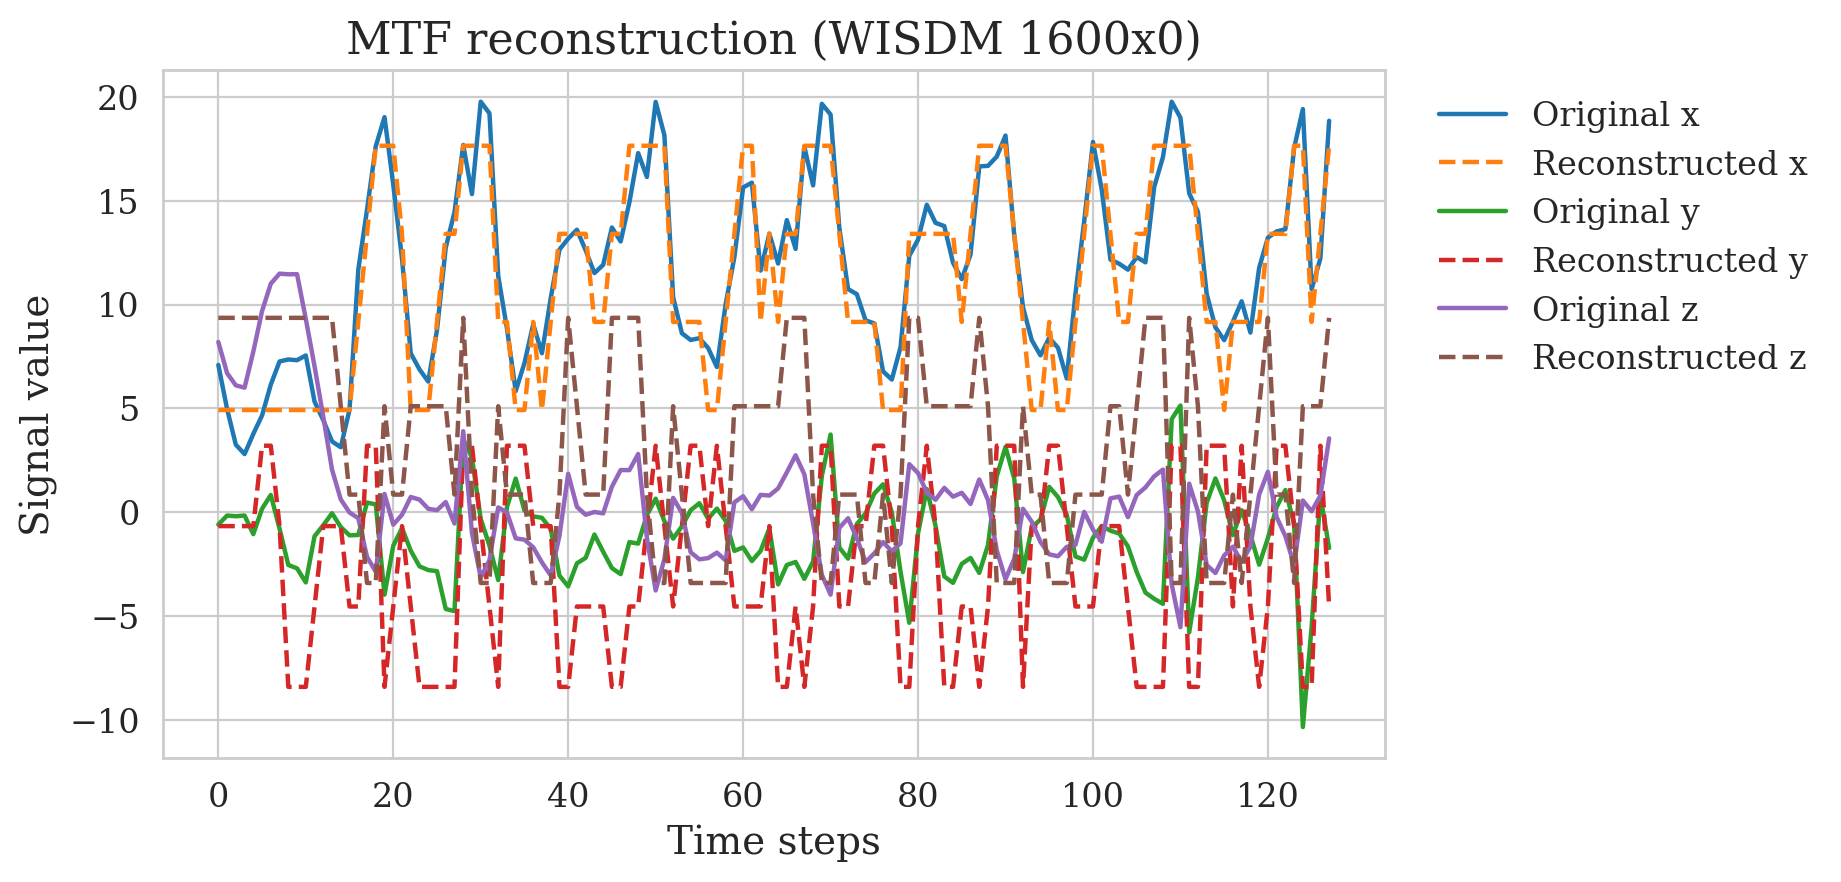
\includegraphics[width=\linewidth]{images/mtf_sample_0_global.png}
\subfigtext{(d) MTF}

\end{minipage}
\caption{Original and reconstructed triaxial signals for one WISDM walking window.}
\label{fig:qualitative_main}
\end{figure*}

\subsection{Reconstruction fidelity}

Table~\ref{tab:pointwise_pooled} reports pooled pointwise fidelity in physical units and Table~\ref{tab:fidelity_spectral} the range-normalised and spectral metrics. Each deterministic decoder scores every one of the 8,172 windows once, so the pooled values are identical for the window-level and subject-out partitions. RP, GASF, and GADF operate near the 8-bit image-quantisation floor under their stated metadata contracts, whereas MTF is orders of magnitude less accurate pointwise. On average, the near-original trio also preserves spectral shape (mean distance below 0.01) and dominant frequency (mean error below 0.01\,Hz); the nonzero standard deviations in Table~\ref{tab:fidelity_spectral} show that these are aggregate statements rather than bounds for every window. MTF's mean spectral-shape distance is 0.362 and its mean dominant-frequency error is 0.573\,Hz. The local-change error \(\Delta\)-NMAE stays at the \(10^{-3}\) level for the near-original methods and rises to 0.202 for MTF.

\begin{table}[!htbp]
\centering
\caption{Pooled pointwise fidelity over 8,172 windows, physical units (m/s\(^2\)).}
\label{tab:pointwise_pooled}
\begin{tabular}{lccc}
\toprule
Method & MAE (mean \(\pm\) std) & MSE & Pearson \\
\midrule
RP   & \(0.0148\pm0.0170\) & 0.0010 & 0.99998 \\
GASF & \(0.0205\pm0.0199\) & 0.0043 & 0.99988 \\
GADF & \(0.0157\pm0.0167\) & 0.0008 & 0.99999 \\
MTF  & \(3.94\pm4.25\)     & 55.43  & 0.01356 \\
\bottomrule
\end{tabular}
\end{table}

\begin{table*}[!htbp]
\centering
\caption{Range-normalised and spectral fidelity over 8,172 windows (mean\(\pm\)std across windows, averaged over the three axes). PSD-shape distance compares Welch spectra after each is normalised to unit mass; energy and band-mass errors are reported separately in the Supplementary Material.}
\label{tab:fidelity_spectral}
\resizebox{\textwidth}{!}{%
\begin{tabular}{lcccccc}
\toprule
Method & NMAE & NRMSE & Pearson & \(\Delta\)-NMAE & PSD-shape dist. & Dom.-freq.\ err.\ (Hz) \\
\midrule
RP   & \(0.0011\pm0.0007\) & \(0.0013\pm0.0009\) & \(0.99998\pm0.00005\) & \(0.0011\pm0.0008\) & \(0.0018\pm0.0018\) & \(0.001\pm0.035\) \\
GASF & \(0.0015\pm0.0006\) & \(0.0028\pm0.0012\) & \(0.99988\pm0.00014\) & \(0.0021\pm0.0007\) & \(0.0071\pm0.0051\) & \(0.007\pm0.085\) \\
GADF & \(0.0013\pm0.0005\) & \(0.0014\pm0.0006\) & \(0.99999\pm0.00001\) & \(0.0009\pm0.0003\) & \(0.0026\pm0.0019\) & \(0.005\pm0.081\) \\
MTF  & \(0.278\pm0.080\)   & \(0.326\pm0.091\)   & \(0.014\pm0.489\)     & \(0.202\pm0.069\)   & \(0.362\pm0.181\)   & \(0.573\pm1.111\) \\
\bottomrule
\end{tabular}
}
\end{table*}

Paired window-level Wilcoxon tests distinguish every encoder pair after Holm correction. The practically important effect is the separation from MTF: RP, GASF, and GADF each show a large effect (\(|r|=0.866\)) against it. Differences within the near-original trio are small in absolute units despite statistical detection at \(N=8{,}172\). Repeating the test on 51 subject means preserves the MTF separation and the modest GADF-over-GASF ordering, showing that these findings are not produced solely by window-level pseudoreplication. Per-fold and per-axis breakdowns, and the full per-classifier subject-clustered equivalence under both protocols, are in the Supplementary Material.

\subsection{Robustness to image perturbation}
\label{sec:results_robustness}

The implementation follows the local-stability protocol defined above. The activity-balanced sample contains 30 windows per class and covers all 51 subjects. The self-consistency objects are the newly decoded clean reconstruction \(\hat x^{(0)}_{m,w}\) and its cached pipeline counterpart \(\hat x^{\mathrm{cache}}_{m,w}\); all four methods passed the per-window gate.

Table~\ref{tab:robustness} shows increasing error for the three near-original decoders, but no catastrophic failure within the tested range: at \(\sigma=16\) (about \(6\%\) of the intensity range), their mean NMAE remains below \(0.07\). RP has the lowest descriptive mean at every nonzero level (\(0.034\) at \(\sigma=16\)), followed by GASF (\(0.063\)) and GADF (\(0.067\)); this experiment was not designed as a pairwise superiority test, so we do not infer a population-level robustness ranking from those means alone. MTF stays near \(0.28\) across the curve because its representative reconstruction is already dominated by intrinsic quantisation loss. Subject-cluster intervals and cycle residuals are reported in the Supplementary Material. These results quantify local stability only; they do not cover the coherent structural defects of generated images.

\begin{table*}[!htbp]
\centering
\caption{Controlled local-stability test: NMAE under zero-mean Gaussian pixel noise (standard deviation \(\sigma\), out of 255). Values are mean$\pm$standard deviation across 150 activity-balanced, subject-spread windows after averaging two independent draws per nonzero level. Subject-cluster 95\% intervals are in the Supplementary Material.}
\label{tab:robustness}
\resizebox{\textwidth}{!}{%
\begin{tabular}{lccccc}
\toprule
Method & \(\sigma=0\) & \(\sigma=2\) & \(\sigma=4\) & \(\sigma=8\) & \(\sigma=16\) \\
\midrule
RP   & $0.0011\pm0.0007$ & $0.0045\pm0.0030$ & $0.0084\pm0.0050$ & $0.0170\pm0.0090$ & $0.0340\pm0.0143$ \\
GASF & $0.0015\pm0.0003$ & $0.0130\pm0.0043$ & $0.0214\pm0.0053$ & $0.0358\pm0.0061$ & $0.0634\pm0.0084$ \\
GADF & $0.0012\pm0.0004$ & $0.0074\pm0.0018$ & $0.0147\pm0.0031$ & $0.0315\pm0.0079$ & $0.0669\pm0.0161$ \\
MTF  & $0.2812\pm0.0836$ & $0.2845\pm0.0850$ & $0.2868\pm0.0818$ & $0.2838\pm0.0787$ & $0.2797\pm0.0751$ \\
\bottomrule
\end{tabular}
}
\end{table*}

The Supplementary Material attributes error to the native floating-operator inverse, the clean 8-bit round trip, and perturbed storage. That decomposition resolves the apparent GADF contradiction: its native float inverse is exact, whereas the small nonzero term previously called ``float error'' included the storage mapping. For the near-original methods, 8-bit quantisation is the dominant clean-round-trip source; it is not the only source for RP. MTF's loss is already present in its floating representative reconstruction.

\subsection{Downstream classification}
\label{sec:subject_out_results}

Table~\ref{tab:subject_out_acc} is the main classification result, under the primary grouped subject-out protocol. RP, GASF, and GADF track the original signal on every classifier, while MTF degrades all of them. The corresponding within-distribution window-level accuracies --- uniformly higher, as expected --- and all six classifiers are reported in the Supplementary Material; the ranking is identical under both protocols.

\begin{table}[!htbp]
\centering
\caption{Grouped subject-out three-fold accuracy (primary protocol) for three representative classifiers spanning the families (convolutional, recurrent, classical). All six classifiers and the window-level comparison are in the Supplementary Material.}
\label{tab:subject_out_acc}
\begin{tabular}{lccccc}
\toprule
Classifier & Original & RP & GASF & GADF & MTF \\
\midrule
CNN & 0.794 & 0.794 & 0.794 & 0.794 & 0.684 \\
GRU & 0.811 & 0.811 & 0.811 & 0.811 & 0.702 \\
RF  & 0.786 & 0.786 & 0.787 & 0.787 & 0.689 \\
\bottomrule
\end{tabular}
\end{table}

McNemar difference tests are secondary because failure to reject a difference does not establish equivalence. The primary result is Table~\ref{tab:equivalence_ci}: each classifier-specific simultaneous interval lies within \(\pm0.01\) for RP, GASF, and GADF, even when complete subjects are held out. The table compresses those intervals by displaying their total span; that span is a descriptive summary, not itself a confidence interval. All 24 individual simultaneous intervals are shown in the Supplementary Material. Holm-adjusted TOST gives the same method-level verdict. MTF is equivalent to none: its mean per-subject accuracy deficit ranges from 0.05 to 0.11 under subject-out.

\begin{table*}[!htbp]
\centering
\caption{Subject-level classification equivalence under grouped subject-out validation. The primary family comprises 18 simultaneous subject-cluster bootstrap intervals (six classifiers by RP/GASF/GADF); the six MTF negative-control comparisons form a separate family (51 subjects, \(10^4\) joint resamples per family). ``Interval span'' is descriptive; individual intervals are in the Supplementary Material.}
\label{tab:equivalence_ci}
\begin{tabular}{lcccc}
\toprule
Method & Mean \(\Delta\)acc range & Simultaneous 95\% interval span & Equiv.\ \(\pm0.01\) & Equiv.\ \(\pm0.02\) \\
\midrule
RP   & \([-0.0002,+0.0012]\) & \([-0.0023,+0.0033]\) & 6/6 & 6/6 \\
GASF & \([-0.0006,+0.0000]\) & \([-0.0027,+0.0021]\) & 6/6 & 6/6 \\
GADF & \([-0.0005,+0.0008]\) & \([-0.0027,+0.0030]\) & 6/6 & 6/6 \\
MTF  & \([+0.047,+0.112]\)   & \([+0.0209,+0.1389]\) & 0/6 & 0/6 \\
\bottomrule
\end{tabular}
\end{table*}

\subsection{Decoder ablations}
\label{sec:decoder_ablation}

Table~\ref{tab:ablation_summary} retains only the decision-changing ablations. Both RP geometry choices are necessary; GADF benefits from pivot averaging; and spectral ordering improves the MTF representative without making it faithful. The raw floating-operator GADF inverse is exact to numerical precision (MAE \(<10^{-6}\)); the earlier nonzero ``float'' value arose from applying the fixed storage map before decoding, not from the operator inverse. Full sweeps, runtime, anchor failures, and the float/PNG decomposition are in the Supplementary Material.

\begin{table*}[!htbp]
\centering
\caption{Compact decoder-ablation summary. MAE is in physical units (m/s\(^2\)); datasets differ by method as detailed in the Supplementary Material.}
\label{tab:ablation_summary}
\small
\begin{tabular}{llll}
\toprule
Method & Used variant (MAE) & Degraded alternative (MAE) & Interpretation \\
\midrule
RP & 2-D MDS + signed (0.010) & wrong RP range (1.047) & operator scale is essential \\
GADF & five pivots (0.0158) & one pivot (0.0353) & averaging suppresses PNG noise \\
MTF & Fiedler (5.060) & cosine pivot (6.493) & improved but intrinsically lossy \\
\bottomrule
\end{tabular}
\end{table*}

\section{Discussion}
\label{sec:discussion}

\subsection{Interpretation of the comparison}
\label{sec:disc_pointwise}

The fidelity and utility blocks support one consistent division. RP, GASF, and GADF reconstruct near the 8-bit storage floor, preserve spectral shape on average, and remain equivalent to the raw signal for original-trained classification under both validation protocols. MTF is worse on every block. Classification alone would not establish reconstruction fidelity: a coarse representation can retain class information while losing amplitude. Here the pointwise and spectral metrics show that the three leading methods recover the signal under their stated contracts, whereas MTF preserves only a quantile-transition summary.

The small ordering among RP, GADF, and GASF should not obscure this result. RP has the lowest observed mean MAE, GADF the lowest MSE and highest Pearson correlation, and GASF the simplest established inverse. Their absolute differences are tiny compared with the gap to MTF, and no corresponding classification separation is detected.

Practically, GASF is the simplest faithful baseline; GADF provides directional-difference recovery under a restricted branch; and RP preserves recurrence geometry at the cost of method-specific operator-range metadata and MDS. MTF is appropriate only when a coarse transition summary is acceptable. Holding out complete subjects reduces absolute classifier accuracy but does not alter this grouping. The simultaneous subject-cluster intervals turn a non-significant difference into a positive, margin-relative equivalence statement for RP, GASF, and GADF; TOST agrees.

\subsection{Relationship between signed RP and GADF}
\label{sec:disc_structural}

Signed RP and GADF are not equivalent matrices, but both encode directional pairwise differences. For slowly varying local increments,
\[
R_{ij}\approx \sigma(i,j)\sqrt2\,|x_i-x_j|,
\qquad
G^{\mathrm D}_{ij}\approx
\frac{\bar x_j-\bar x_i}{\sqrt{1-\bar x^2}}.
\]
GADF is intrinsically antisymmetric because its sign follows from \(\sin(\phi_i-\phi_j)\); the Lu--Tong RP applies an external directional sign and need not be exactly antisymmetric. This analogy explains their visual proximity without implying a shared inverse or formal information equivalence. The full operator derivation and null-corrected regional-overlap diagnostic are provided in the Supplementary Material.

\subsection{Limitations and scope}
\label{sec:disc_scope}

\begin{itemize}
\item \textbf{Controlled inputs.} Every image is produced by a known encoder. The repeated Gaussian-noise experiment measures only local pixel stability; it does not cover structural invalidity, occlusion, missing anchors, non-Euclidean RP matrices, or genuinely generated images. Augmentation benefit is therefore not demonstrated.
\item \textbf{Metadata and scale.} RP needs its per-window operator range even for normalised reconstruction and cannot be recovered from the image alone. All methods need common amplitude calibration only for physical-unit output. The headline values therefore compare declared method contracts, not equal side information, and generated images would require a mechanism to supply or predict that metadata. Part of this cost is dataset-induced rather than intrinsic: because the WISDM sensor full-scale range is undocumented, the common calibration uses each window's observed \((x_{\min},x_{\max})\). A known full-scale range would reduce that calibration to a global constant and, combined with a fixed RP storage range in place of the per-window min--max convention, would remove RP's per-window metadata dependence and place it on the same image-only footing as GASF and GADF --- at some 8-bit quantisation cost for low-amplitude windows.
\item \textbf{Branch and anchor assumptions.} GASF uses a fixed branch; GADF requires \(\alpha<1/\sqrt2\), a consistent sign convention, and a detectable boundary. Near-constant or perturbed images may violate the anchor assumption.
\item \textbf{Statistical dependence.} Pooled window tests understate intra-subject dependence and combine fold-specific rules. The primary intervals resample subjects jointly and control the 18-comparison subject-out family; MTF is handled as a separate six-comparison negative-control family. Equivalence remains relative to the chosen margin. The \(\pm0.02\) result is only a less stringent sensitivity analysis.
\item \textbf{MTF tuning.} The exploratory \(Q\) sweep used pooled test data; MTF is therefore a descriptive lossy control, not a confirmatorily tuned competitor. Nested subject-grouped selection is still required for that comparison.
\item \textbf{External validity.} Results cover one smartwatch accelerometer dataset, five activities, 51 subjects, 20\,Hz sampling, and \(N=128\) windows.
\item \textbf{Storage precision.} The near-original tier is measured after an 8-bit PNG round trip; other formats or perturbations may change the error floor.
\end{itemize}

\subsection{Reproducibility}
\label{sec:reproducibility}

The implementation uses Python 3.10--3.11, TensorFlow 2.11--2.15, scikit-learn, and SciPy. Classical MDS is deterministic; reconstructed windows retain explicit indices during parallel execution; and both fold assignments use fixed seeds. The repository includes encoders, decoders, classifiers, the fidelity and spectral metric module, the subject-clustered equivalence and bootstrap tests, and the table-generation scripts. Extended configurations and outputs are supplied in the Supplementary Material.

\section{Conclusion}
\label{sec:conclusion}

We presented two faithful reconstruction methods for image-based time-series representations: a two-dimensional signed-RP decoder and a restricted-branch, boundary-anchored GADF decoder. The GASF diagonal decoder served as the prior-art invertible baseline, while the many-to-one Fiedler MTF decoder served as a best-effort lossy control. All four were evaluated on the same 8,172 WISDM windows, with the same reconstruction metrics and six original-trained classifiers under both window-level and grouped subject-out validation.

Under their declared encoder--decoder contracts, RP, GASF, and GADF form one near-original tier. Their mean MAEs are 0.0148, 0.0205, and 0.0157\,m/s$^2$; their mean temporal correlations are approximately one; and their mean spectral-shape and dominant-frequency errors are small, with between-window dispersion reported explicitly. Their classifier accuracies are equivalent to the raw signal within a one-percentage-point margin under simultaneous subject-cluster bootstrap intervals. They reach this result through different information: RP recovers adjacent-state geometry, GASF uses its diagonal, and GADF uses anchored angular differences. MTF remains many-to-one and consistently lossy.

These conclusions apply to controlled images produced by known encoders. RP requires its stored matrix range, GASF and GADF require fixed angular assumptions, and physical-unit output requires amplitude calibration. The controlled perturbation experiment establishes local stability only. The next step is to evaluate structurally imperfect and genuinely generated images, including failures of the GADF anchor and non-Euclidean RP geometry. A subsequent train--test transfer matrix will then determine whether reconstructed synthetic windows provide measurable augmentation value.


\begin{thebibliography}{99}

\bibitem{eckmann1995recurrence}
Jean-Pierre Eckmann, S. Oliffson Kamphorst, and David Ruelle. ``Recurrence plots of dynamical systems.'' \textit{Europhysics Letters}, vol. 4, no. 9, pp. 973--977, 1987.


\bibitem{takens1981detecting}
Floris Takens. ``Detecting strange attractors in turbulence.'' In \textit{Dynamical Systems and Turbulence, Warwick 1980}, Lecture Notes in Mathematics, vol. 898, pp. 366--381, Springer, 1981.

\bibitem{marwan2007recurrence}
Norbert Marwan, M. Carmen Romano, Marco Thiel, and Jürgen Kurths. ``Recurrence plots for the analysis of complex systems.'' \textit{Physics Reports}, vol. 438, no. 5--6, pp. 237--329, 2007.

\bibitem{lu2019robust}
Jianjie Lu and Kai-Yu Tong. ``Robust single accelerometer-based activity recognition using modified recurrence plot.'' \textit{IEEE Sensors Journal}, vol. 19, no. 15, pp. 6317--6324, 2019.

\bibitem{hirata2008reproduction}
Yoshito Hirata, Shunsuke Horai, and Kazuyuki Aihara. ``Reproduction of distance matrices and original time series from recurrence plots and their applications.'' \textit{The European Physical Journal Special Topics}, vol. 164, no. 1, pp. 13--22, 2008.

\bibitem{sipers2011unique}
Aloys Sipers, Paul J. A. Borm, and Ralf L. M. Peeters.
``On the unique reconstruction of a signal from its unthresholded recurrence plot.''
\textit{Physics Letters A}, vol. 375, no. 24, pp. 2309--2321, 2011.
doi: \url{https://doi.org/10.1016/j.physleta.2011.04.040}.

\bibitem{sipers2017robust}
Aloys Sipers, Paul J. A. Borm, and Ralf L. M. Peeters.
``Robust reconstruction of a signal from its unthresholded recurrence plot subject to disturbances.''
\textit{Physics Letters A}, vol. 381, no. 6, pp. 604--615, 2017.
doi: \url{https://doi.org/10.1016/j.physleta.2016.12.028}.

\bibitem{wang2015encoding}
Zhiguang Wang and Tim Oates. ``Imaging time-series to improve classification and imputation.'' In \textit{Proceedings of the 24th International Joint Conference on Artificial Intelligence (IJCAI)}, pp. 3939--3945, 2015.

\bibitem{wang2015encoding2}
Zhiguang Wang and Tim Oates. ``Encoding time series as images for visual inspection and classification using tiled convolutional neural networks.'' In \textit{Workshops at the Twenty-Ninth AAAI Conference on Artificial Intelligence}, 2015.

\bibitem{huamin2020reconstruction}
Huamin Tao, Qiuqun Deng, and Shanzhu Xiao. ``Reconstruction of time series with missing value using 2D representation-based denoising autoencoder.'' \textit{Journal of Systems Engineering and Electronics}, vol. 31, no. 6, pp. 1087--1096, 2020.

\bibitem{ahmad2021inertial}
Zeeshan Ahmad and Naimul Khan.
``Inertial Sensor Data to Image Encoding for Human Action Recognition.''
\textit{IEEE Sensors Journal},
vol. 21, no. 9, pp. 10978--10988, 2021.
doi: \url{https://doi.org/10.1109/JSEN.2021.3062261}.

\bibitem{ma2024anomaly}
Jidong Ma and Hairu Wang.
``Anomaly detection in sensor data via encoding time series into images.''
\textit{Journal of King Saud University -- Computer and Information Sciences},
vol. 36, no. 10, article 102232, 2024.
doi: \url{https://doi.org/10.1016/j.jksuci.2024.102232}.

\bibitem{huang2023tsdigan}
Tongge Huang, Pranamesh Chakraborty, and Anuj Sharma.
``Deep convolutional generative adversarial networks for traffic data imputation encoding time series as images.''
\textit{International Journal of Transportation Science and Technology},
vol. 12, no. 1, pp. 1--18, 2023.
doi: \url{https://doi.org/10.1016/j.ijtst.2021.10.007}.

\bibitem{hellermann2026imagegan}
Justin Hellermann and Stefan Lessmann.
``Leveraging image-based generative adversarial networks for time series generation.''
\textit{International Journal of Forecasting},
vol. 42, no. 2, pp. 616--639, 2026.
doi: \url{https://doi.org/10.1016/j.ijforecast.2025.09.004}.

\bibitem{kopec1994document}
Gary E. Kopec and Philip A. Chou. ``Document image decoding using Markov source models.'' \textit{IEEE Transactions on Pattern Analysis and Machine Intelligence}, vol. 16, no. 6, pp. 602--617, 1994.

\bibitem{kliewer2006iterative}
Jörg Kliewer, Norbert Goertz, and Alfred Mertins. ``Iterative source-channel decoding with Markov random field source models.'' \textit{IEEE Transactions on Signal Processing}, vol. 54, no. 10, pp. 3688--3701, 2006.


\bibitem{misc_wisdm_smartphone_and_smartwatch_activity_and_biometrics_dataset__507}
Gary Weiss. ``WISDM Smartphone and Smartwatch Activity and Biometrics Dataset.'' \textit{UCI Machine Learning Repository}, 2019. doi: \url{https://doi.org/10.24432/C5HK59}.

\bibitem{Atkins1998}
Jonathan E. Atkins, Erik G. Boman, and Bruce Hendrickson.
``A spectral algorithm for seriation and the consecutive ones problem.''
\textit{SIAM Journal on Computing}, vol. 28, no. 1, pp. 297--310, 1998. doi: \url{https://doi.org/10.1137/S0097539795285771}.

\bibitem{Wilcoxon1945}
Frank Wilcoxon. ``Individual comparisons by ranking methods.'' \textit{Biometrics Bulletin}, vol. 1, no. 6, pp. 80--83, 1945.

\bibitem{Welch1967}
Peter D. Welch. ``The use of fast Fourier transform for the estimation of power spectra: A method based on time averaging over short, modified periodograms.'' \textit{IEEE Transactions on Audio and Electroacoustics}, vol. 15, no. 2, pp. 70--73, 1967. doi: \url{https://doi.org/10.1109/TAU.1967.1161901}.

\bibitem{McNemar1947}
Quinn McNemar. ``Note on the sampling error of the difference between correlated proportions or percentages.'' \textit{Psychometrika}, vol. 12, no. 2, pp. 153--157, 1947. doi: \url{https://doi.org/10.1007/BF02295996}.

\bibitem{DavisonHinkley1997}
Anthony C. Davison and David V. Hinkley. \textit{Bootstrap Methods and Their Application}. Cambridge University Press, 1997.

\bibitem{Schuirmann1987}
Donald J. Schuirmann. ``A comparison of the two one-sided tests procedure and the power approach for assessing the equivalence of average bioavailability.'' \textit{Journal of Pharmacokinetics and Biopharmaceutics}, vol. 15, no. 6, pp. 657--680, 1987. doi: \url{https://doi.org/10.1007/BF01068419}.

\bibitem{Lakens2017}
Daniël Lakens. ``Equivalence tests: A practical primer for t tests, correlations, and meta-analyses.'' \textit{Social Psychological and Personality Science}, vol. 8, no. 4, pp. 355--362, 2017. doi: \url{https://doi.org/10.1177/1948550617697177}.


\bibitem{Holm1979}
Sture Holm. ``A simple sequentially rejective multiple test procedure.'' \textit{Scandinavian Journal of Statistics}, vol. 6, no. 2, pp. 65--70, 1979.
\end{thebibliography}
\end{document}
